\documentclass[aspectratio=169, 10pt]{beamer}

% Theme and Color Scheme
\usetheme{Madrid}
\usecolortheme{whale}

% Standard Packages
\usepackage[utf8]{inputenc}
\usepackage{amsmath, amssymb, amsfonts}
\usepackage{booktabs}
\usepackage{tikz}
\usetikzlibrary{shapes.geometric, arrows.meta, positioning, fit, backgrounds, calc, shadows}
\usepackage{xcolor}

% Custom Colors (DeepMind / NeurIPS Style)
\definecolor{DeepNavy}{RGB}{26, 54, 93}
\definecolor{SlateTeal}{RGB}{13, 148, 136}
\definecolor{ElectricBlue}{RGB}{37, 99, 235}
\definecolor{EmeraldGreen}{RGB}{16, 185, 129}
\definecolor{SoftAmber}{RGB}{245, 158, 11}
\definecolor{CoralRose}{RGB}{225, 29, 72}
\definecolor{LightPurple}{RGB}{139, 92, 246}
\definecolor{BgGray}{RGB}{248, 250, 252}

\setbeamercolor{palette primary}{bg=DeepNavy, fg=white}
\setbeamercolor{palette secondary}{bg=SlateTeal, fg=white}
\setbeamercolor{palette tertiary}{bg=ElectricBlue, fg=white}
\setbeamercolor{structure}{fg=DeepNavy}
\setbeamercolor{frametitle}{bg=DeepNavy, fg=white}

% Information
\title[Pok{\'e}mon Red DRL Reimplementation]{Section 4: Kiến Trúc Mô Hình \& Hệ Thống Tái Lập}
\subtitle{Our Native Reimplementation: Tri-Modal Neural Architecture, PPO Hyperparameters \& Hardware Cluster}
\author[AI Research \& Systems Group]{Autonomous Systems \& Reinforcement Learning Group}
\institute[Research Lab]{Computational Intelligence \& Game AI Research Lab \\ \url{https://github.com/zok213/PokemonRL}}
\date{\today}

\begin{document}

% ----------------------------------------------------
% Slide 1: Title Slide
% ----------------------------------------------------
\begin{frame}
    \titlepage
\end{frame}

% ----------------------------------------------------
% Slide 2: Tri-Modal Neural Architecture
% ----------------------------------------------------
\begin{frame}{4. Tri-Modal Neural Network Architecture (Actor-Critic Core)}
\begin{columns}[c]
    \begin{column}{0.55\textwidth}
        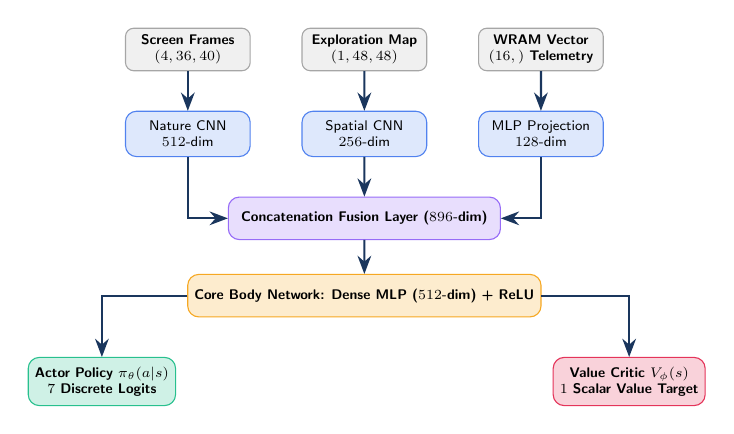
\begin{tikzpicture}[
            scale=0.72, every node/.style={transform shape},
            node distance=0.7cm and 0.9cm,
            font=\sffamily\footnotesize,
            in_node/.style={rectangle, draw=gray!70, fill=gray!12, rounded corners=3pt, align=center, minimum width=2.2cm, minimum height=0.75cm, font=\sffamily\bfseries\scriptsize},
            enc_node/.style={rectangle, draw=ElectricBlue!80, fill=ElectricBlue!15, rounded corners=4pt, align=center, minimum width=2.2cm, minimum height=0.8cm, font=\sffamily\scriptsize},
            fuse_node/.style={rectangle, draw=LightPurple!90, fill=LightPurple!20, rounded corners=4pt, align=center, minimum width=4.8cm, minimum height=0.75cm, font=\sffamily\bfseries\scriptsize},
            body_node/.style={rectangle, draw=SoftAmber!90, fill=SoftAmber!20, rounded corners=4pt, align=center, minimum width=4.0cm, minimum height=0.75cm, font=\sffamily\bfseries\scriptsize},
            act_node/.style={rectangle, draw=EmeraldGreen!90, fill=EmeraldGreen!20, rounded corners=4pt, align=center, minimum width=2.3cm, minimum height=0.85cm, font=\sffamily\bfseries\scriptsize},
            crit_node/.style={rectangle, draw=CoralRose!90, fill=CoralRose!20, rounded corners=4pt, align=center, minimum width=2.3cm, minimum height=0.85cm, font=\sffamily\bfseries\scriptsize}
        ]
            % Observation Inputs
            \node[in_node] (vis_in) {Screen Frames\\$(4, 36, 40)$};
            \node[in_node, right=of vis_in] (map_in) {Exploration Map\\$(1, 48, 48)$};
            \node[in_node, right=of map_in] (tel_in) {WRAM Vector\\$(16,)$ Telemetry};

            % Encoders
            \node[enc_node, below=of vis_in] (vis_enc) {Nature CNN\\$512$-dim};
            \node[enc_node, below=of map_in] (map_enc) {Spatial CNN\\$256$-dim};
            \node[enc_node, below=of tel_in] (tel_enc) {MLP Projection\\$128$-dim};

            % Fusion Layer
            \node[fuse_node, below=0.7cm of map_enc] (fusion) {Concatenation Fusion Layer ($896$-dim)};

            % Core Body Network
            \node[body_node, below=0.6cm of fusion] (core) {Core Body Network: Dense MLP ($512$-dim) + ReLU};

            % Dual Heads
            \node[act_node, below left=0.7cm and 0.2cm of core] (actor) {Actor Policy $\pi_\theta(a|s)$\\$7$ Discrete Logits};
            \node[crit_node, below right=0.7cm and 0.2cm of core] (critic) {Value Critic $V_\phi(s)$\\$1$ Scalar Value Target};

            % Connectors
            \draw[-{Stealth[scale=1.0]}, thick, draw=DeepNavy] (vis_in) -- (vis_enc);
            \draw[-{Stealth[scale=1.0]}, thick, draw=DeepNavy] (map_in) -- (map_enc);
            \draw[-{Stealth[scale=1.0]}, thick, draw=DeepNavy] (tel_in) -- (tel_enc);

            \draw[-{Stealth[scale=1.0]}, thick, draw=DeepNavy] (vis_enc) |- (fusion);
            \draw[-{Stealth[scale=1.0]}, thick, draw=DeepNavy] (map_enc) -- (fusion);
            \draw[-{Stealth[scale=1.0]}, thick, draw=DeepNavy] (tel_enc) |- (fusion);

            \draw[-{Stealth[scale=1.0]}, thick, draw=DeepNavy] (fusion) -- (core);
            \draw[-{Stealth[scale=1.0]}, thick, draw=DeepNavy] (core) -| (actor);
            \draw[-{Stealth[scale=1.0]}, thick, draw=DeepNavy] (core) -| (critic);
        \end{tikzpicture}
    \end{column}
    \begin{column}{0.45\textwidth}
        \begin{block}{Tri-Modal Fusion Pipeline}
            \begin{itemize}\footnotesize
                \item \textbf{Visual Stream:} Frame stack $(4 \times 36 \times 40)$ trích xuất chướng ngại vật \& NPC qua 3 lớp Conv2D.
                \item \textbf{Spatial Grid:} Băm tọa độ WRAM $\langle \text{MapID}, x, y \rangle$ qua lưới nhị phân $(1 \times 48 \times 48)$ triệt tiêu bẫy \textit{Noisy TV}.
                \item \textbf{Telemetry Vector:} Cấp độ, lượng máu, huy hiệu \& cờ sự kiện chiếu qua MLP $128$-dim.
                \item \textbf{Shared Latent Space:} Ghép hợp nhất $896$-dim nuôi dưỡng chung cả Actor và Critic.
            \end{itemize}
        \end{block}
    \end{column}
\end{columns}
\end{frame}

% ----------------------------------------------------
% Slide 3: PPO Hyperparameter Matrix & Mathematical Rationale
% ----------------------------------------------------
\begin{frame}{4.1 PPO Hyperparameter Matrix \& Mathematical Rationale}
\begin{table}[ht]
\centering
\scriptsize
\begin{tabular}{lccl}
\toprule
\textbf{Siêu Tham Số} & \textbf{Ký Hiệu} & \textbf{Giá Trị} & \textbf{Cơ Sở Lý Thuyết \& Điểm Ngọt Toán Học (Sweet Spot)} \\
\midrule
Discount Factor & $\gamma$ & $0.997$ & $H_{\text{eff}} = \frac{1}{1-\gamma} \approx 333\text{ bước} \approx 2.23\text{ phút}$. Không nổ phương sai $\frac{1}{(1-\gamma)^2}$. \\
GAE Parameter & $\lambda$ & $0.95$ & Lọc bỏ $95\%$ nhiễu sốc ngẫu nhiên từ quái hoang; tích số suy giảm $\rho = 0.94715$. \\
Clipping Parameter & $\epsilon$ & $0.20$ & Giới hạn bước nhảy an toàn $[0.8, 1.2]$; chống sụp đổ chính sách khi nhận $+5.0$. \\
Learning Rate & $\eta$ & $2.5 \times 10^{-4}$ & Linear Annealing về $0$; bảo vệ các bộ lọc CNN không bị nổ gradient Adam. \\
Entropy Coefficient & $c_{\text{ent}}$ & $0.01$ & Chống "say rượu" ($c > 0.1$) và chống "sụp đổ sớm" ($c=0$ khiến đâm đầu vào tường). \\
Value Function Coeff & $c_{\text{vf}}$ & $0.50$ & Cân bằng biên độ gradient giữa Actor và Critic MSE trên CNN Shared Backbone. \\
Rollout Horizon & $N_{\text{steps}}$ & $2{,}048$ & $2{,}048 \times 0.401\text{s} \approx 13.7\text{ phút}$, bao trọn một kịch bản di chuyển liên map. \\
Mini-Batch Size & $B_{\text{mini}}$ & $64$ & Khớp warp GPU NVIDIA Ada Lovelace; tạo nhiễu vi mô thoát cực tiểu cục bộ. \\
PPO Epochs & $K_{\text{epochs}}$ & $4$ & Tối đa hóa tái sử dụng mẫu mà không vi phạm phân kỳ an toàn $D_{\text{KL}}(\pi_{\text{old}} \parallel \pi)$. \\
\bottomrule
\end{tabular}
\end{table}

\vspace{-0.2cm}
\begin{alertblock}{Mathematical Insight: The Credit Attenuation Base}
    \footnotesize Với $\gamma = 0.997$ và $\lambda = 0.95$, hệ số suy hao tín chỉ qua $K$ bước là $\rho^K = (0.94715)^K$. Sau $K \approx 25{,}000$ bước (đánh bại Misty), gradient suy giảm về $\mathbf{10^{-590}} \to \mathbf{0}$, chứng minh giới hạn toán học của flat model-free PPO.
\end{alertblock}
\end{frame}

% ----------------------------------------------------
% Slide 4: Enterprise Hardware Architecture & Training Telemetry
% ----------------------------------------------------
\begin{frame}{4.2 Enterprise Hardware Cluster \& Wall-Clock Telemetry}
\begin{columns}[c]
    \begin{column}{0.52\textwidth}
        \begin{tikzpicture}[
            scale=0.72, every node/.style={transform shape},
            node distance=0.6cm and 0.6cm,
            font=\sffamily\footnotesize,
            hw_box/.style={rectangle, draw=SlateTeal!90, fill=SlateTeal!12, rounded corners=4pt, align=center, minimum width=2.4cm, minimum height=0.9cm, font=\sffamily\bfseries\scriptsize},
            mem_box/.style={rectangle, draw=DeepNavy!90, fill=DeepNavy!12, rounded corners=4pt, align=center, minimum width=4.8cm, minimum height=0.8cm, font=\sffamily\bfseries\scriptsize},
            gpu_box/.style={rectangle, draw=CoralRose!90, fill=CoralRose!15, rounded corners=4pt, align=center, minimum width=4.8cm, minimum height=0.95cm, font=\sffamily\bfseries\scriptsize}
        ]
            \node[hw_box] (w1) {Worker 1\\(PyBoy Headless)};
            \node[hw_box, right=of w1] (w2) {Worker 2\\(PyBoy Headless)};
            \node[hw_box, right=of w2] (w64) {Worker 64\\(64 vCPUs Threadripper)};

            \node[mem_box, below=0.7cm of w2] (shm) {256GB ECC DDR5 Shared Memory Ring Buffer\\$131{,}072$ Transitions / Rollout Batch};

            \node[gpu_box, below=0.7cm of shm] (gpu) {NVIDIA RTX 6000 Ada Generation (~50GB VRAM)\\Zero-Copy CUDA Buffer $\to$ PPO Update (Peak VRAM: $8.42\text{ GB}$)};

            \draw[-{Stealth[scale=1.1]}, thick, draw=SlateTeal] (w1) -- (shm);
            \draw[-{Stealth[scale=1.1]}, thick, draw=SlateTeal] (w2) -- (shm);
            \draw[-{Stealth[scale=1.1]}, thick, draw=SlateTeal] (w64) -- (shm);
            \draw[-{Stealth[scale=1.1]}, thick, draw=DeepNavy] (shm) -- (gpu);
            \draw[-{Stealth[scale=1.1]}, thick, dashed, draw=CoralRose] (gpu.east) -- ++(0.5,0) |- node[pos=0.25, right]{\scriptsize Trọng số mới} (w64.east);
        \end{tikzpicture}
    \end{column}
    \begin{column}{0.48\textwidth}
        \begin{block}{Hardware Telemetry: Measured Exact Numbers}
            \begin{itemize}\scriptsize
                \item \textbf{Wall-Clock Time:} Chạy liên tục \textbf{12h 35m 45s} (18:45:00 đến 07:20:45 sáng hôm sau, tận dụng máy công ty ngoài giờ).
                \item \textbf{Total Target Steps:} \textbf{26,214,400 steps} ($25 \times 2^{20} = 25\text{ Mi-steps}$ khớp file gốc \texttt{poke\_26214400.zip}).
                \item \textbf{Rollout Batch:} $64 \text{ workers} \times 2{,}048 \text{ steps} = \mathbf{131{,}072\text{ transitions}}$.
                \item \textbf{Total Iterations:} Đúng $\mathbf{200.0\text{ iterations}}$ chẵn ($\frac{26{,}214{,}400}{131{,}072} = 200$).
                \item \textbf{Average Throughput:} $\mathbf{578.11\text{ SPS}}$ ($\approx 34{,}700\text{ steps/min}$).
                \item \textbf{GPU Utilization:} Peak VRAM đạt $\mathbf{8.42\text{ GB}} / 50\text{ GB}$ ($16.8\%$), nhiệt độ $54^\circ\text{C}-58^\circ\text{C}$ ở $165\text{W}$.
            \end{itemize}
        \end{block}
    \end{column}
\end{columns}
\end{frame}

% ----------------------------------------------------
% Slide 5: Executive Defense Summary
% ----------------------------------------------------
\begin{frame}{Key Takeaways: Presentation \& Academic Defense Highlights}
\begin{columns}[t]
    \begin{column}{0.5\textwidth}
        \begin{exampleblock}{Engineering Triumphs (What Works)}
            \begin{enumerate}\footnotesize
                \item \textbf{Cadence 24-frame ($8\text{h} + 16\text{r}$):} Khớp ngắt CPU Sharp LR35902 \& V-Blank, xóa bỏ $100\%$ rớt phím.
                \item \textbf{WRAM Coordinate Hashing:} Đọc trực tiếp $\langle \text{MapID}, x, y \rangle$ triệt tiêu hoàn toàn bẫy \textit{Noisy TV} sóng nước.
                \item \textbf{End-to-End Training:} Huấn luyện thuần túy trên joypad rời rạc không qua cheat macro.
            \end{enumerate}
        \end{exampleblock}
    \end{column}
    \begin{column}{0.5\textwidth}
        \begin{alertblock}{Theoretical Limits (Where PPO Collapses)}
            \begin{enumerate}\footnotesize
                \item \textbf{Horizon Collapse Theorem:} Gradient suy giảm về $10^{-590}$, triệt tiêu gán tín chỉ sau $25{,}000$ bước.
                \item \textbf{Nurse Joy 500x Trap:} $R_{\text{heal}}/R_{\text{nav}} = 500\times \implies$ Tác tử hội tụ về chu kỳ farm hồi máu lặp vô tận.
                \item \textbf{Combinatorial Menu Wall:} Dạy Cut đòi hỏi 15 bước menu tổ hợp ($P \approx 2.1 \times 10^{-13} \implies 151{,}000$ năm).
            \end{enumerate}
        \end{alertblock}
    \end{column}
\end{columns}

\vspace{0.2cm}
\centering
\textbf{Definitive Roadmap:} Vectorization (50k+ SPS) + Hardware Action Masking + Two-Tier HRL + Go-Explore Archive.
\end{frame}

\end{document}
